\documentclass[a4paper,oneside,article,11pt]{memoir}
\usepackage[english]{babel}
\usepackage[utf8]{inputenc}
\usepackage{amsmath,amssymb,amsthm}

% This font looks so good.
\usepackage[sc]{mathpazo}

% Typesetting pseudo-code
\usepackage{algorithm}
\usepackage{algorithmic}
\usepackage{multirow}
% Code comments like [CLRS]
\renewcommand{\algorithmiccomment}[1]{\makebox[5cm][l]{$\triangleright$ \textit{#1}}}
\usepackage{framed,graphicx,xcolor}
\usepackage[font={small,it}]{caption}
\usepackage{listings}
\usepackage{units}

% Relative references
\usepackage{varioref}

\usepackage{hyperref}

\bibliographystyle{alpha}

\title{Range Reporting}
\author{Peter Gabrielsen 20114179 \\
Christoffer Hansen 20114637}
\newcounter{qcounter}
\begin{document}

\begin{titlingpage}
\clearpage

\maketitle
\thispagestyle{empty}

\begin{abstract}
blabla
\end{abstract}
\end{titlingpage}

\pagebreak

\tableofcontents

\pagebreak

\chapter{Introduction}

\chapter{Model of computation}
We will argue the results of this thesis in terms of the external memory model of Aggarwal and Vitter~\cite{Aggarwal:1988/ICS/48529.48535}.
The external memory model (or I/O model) measures the efficiency of an algorithm by counting the total number of reads and writes performed. In detail the model consists of two levels of memory; a bounded internal memory of size $M$ and an unbounded external memory. For a total of $N$ records we define an \textit{IO} operation to the process of transferring $B$ consecutive records between the two levels of memory as depicted in figure~\ref{fig:io_model}. We restrict all computations on records to be done in internal memory. Throughout the thesis we will let $K$ denote the total number of records in the output.

\begin{figure}[h]
	\centering
	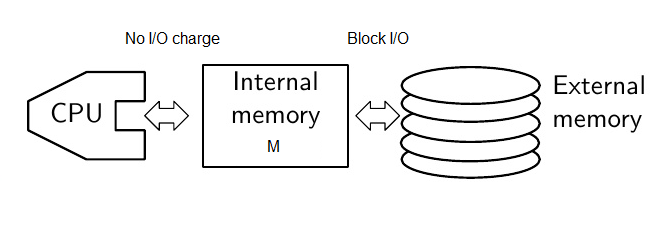
\includegraphics[width=0.8\textwidth]{../figures/io_model.png}
	\caption{The IO Model. Only reads/writes between internal and external memory is charged.}
	\label{fig:io_model}
\end{figure}

The fundamental bounds in the external memory model is that scanning can be done in $\mathcal{O}(\text{Scan}) = \mathcal{O}(\nicefrac{N}{B})$, sorting in $\mathcal{O}(\text{Sort}) = \mathcal{O}(\nicefrac{N}{B} \log_{\nicefrac{M}{B}}\nicefrac{N}{B})$ and searching in $\mathcal{O}(\log_B N)$. We denote $\mathcal{O}(\nicefrac{N}{B})$ as being linear in terms of IOs. Note that the $B$ factor is very important as $\nicefrac{N}{B} < \mathcal{O}(\nicefrac{N}{B} \log_{\nicefrac{M}{B}}\nicefrac{N}{B}) \ll N$.

For convenience we will assume $M > B^2$. This assumption is known as the \textit{tall-cache assumption} in the cache-oblivious model and basically states that the number of blocks \nicefrac{M}{B} is larger than the size of each block $B$~\cite{Prokop99cache-obliviousalgorithms}.

\chapter{Preliminaries}

\section{Amortization}

\section{Global Rebuilding}
The term \textit{global rebuilding} refers to the standard technique of making a (typically small) static data structure dynamic. We simply store all updates in a \textit{update block} and once a certain threshold has been collected we rebuild the data structure~\cite{ionotes}. For data structures that does not allow the space for deleted records to be reoccupied we \textit{mark} (or \textit{weak delete}) the elements. Whenever $\alpha N$ elements have been marked, for some constant $\alpha > 0$, the entire data structure is rebuilt from scratch with only the non-marked elements. The cost of rebuilding is at most a constant factor higher than the cost of inserting $\alpha N$ elements and so the amortized cost of global rebuilding can be charged to the insertions of the deleted elements~\cite{Meyer:2003/AMH/1744652}.

\section{Filtering}
Charge part of query cost to output.

\chapter{Sublogarithmic Updates}

\chapter{External Memory Priority Search Tree}

\bibliography{references}

\end{document}


